\subsection{Winogrande}
{{\footnotesize
\noindent WinoGrande is a large-scale adversarial dataset of 44,000 Winograd Schema-style 
questions with reduced bias using AFLite, serving as both a benchmark and transfer 
learning resource.


\begin{description}[labelwidth=4cm, labelsep=1em, leftmargin=4cm, itemsep=0.1em, parsep=0em]
  \item[date:] 2019-07-24
  \item[version:] 1
  \item[last\_updated:] 2019-07-24
  \item[expired:] false
  \item[valid:] yes
  \item[valid\_date:] 2019-07-24
  \item[url:] \href{https://leaderboard.allenai.org/winogrande/submissions/public}{https://leaderboard.allenai.org/winogrande/submissions/public}
  \item[doi:] 10.48550/arXiv.1907.10641
  \item[domain:] NLP; Commonsense
  \item[focus:] Winograd Schema-style pronoun resolution
  \item[keywords:]
    - adversarial
    - pronoun resolution
  \item[licensing:] CC-BY
  \item[task\_types:]
    - Pronoun resolution
  \item[ai\_capability\_measured:]
    - Robust commonsense reasoning
  \item[metrics:]
    - Accuracy
    - AUC
  \item[models:]
    - RoBERTa
    - BERT
    - GPT-2
  \item[ml\_motif:]
    - Commonsense reasoning
  \item[type:] Benchmark
  \item[ml\_task:]
    - Supervised Learning
  \item[solutions:] 2
  \item[notes:] Human \textasciitilde{}94\%
  \item[contact.name:] Keisuke Sakaguchi
  \item[contact.email:] keisukes@allenai.org
  \item[datasets.links.name:] Hugging Face / AllenAI
  \item[datasets.links.url:] \href{https://huggingface.co/datasets/allenai/winogrande}{https://huggingface.co/datasets/allenai/winogrande}
  \item[results.links.name:] Papers With Code leaderboard
  \item[results.links.url:] \href{https://paperswithcode.com/dataset/winogrande}{https://paperswithcode.com/dataset/winogrande}
  \item[fair.reproducible:] True
  \item[fair.benchmark\_ready:] True
  \item[id:] winogrande
  \item[Citations:] \cite{sakaguchi2019winograndeadversarialwinogradschema}
\end{description}

{\bf Ratings:} ~ \\

\begin{tabular}{p{0.15\textwidth} p{0.07\textwidth} p{0.7\textwidth}}
\hline
Rating & Value & Reason \\
\hline
dataset & 5 & Public, versioned, and FAIR-compliant with AFLite-generated splits to reduce annotation artifacts; hosted by AllenAI with good metadata.
 \\
documentation & 5 & Dataset page and paper provide sufficient detail
 \\
metrics & 5 & Accuracy and AUC are quantitative and well-aligned with disambiguation goals; standardized across evaluations.
 \\
reference\_solution & 4 & Baseline results available, requiring users to submit their methods along with their submissions. Constraints are not required in submissions.
 \\
software & 0 & No template code provided
 \\
specification & 5 & Task (pronoun/coreference resolution) is clearly defined in Winograd Schema style, with consistent input/output format; no system constraints included.
 \\
\hline
\end{tabular}

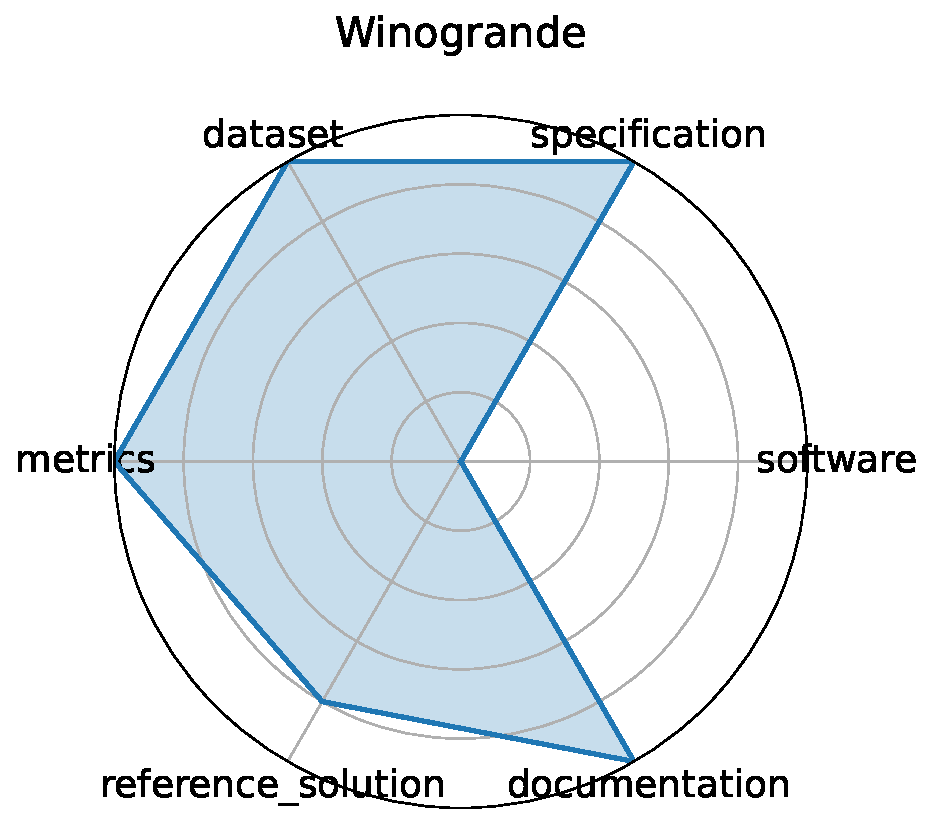
\includegraphics[width=0.2\textwidth]{winogrande_radar.pdf}
}}
\clearpage